En esta imagen se muestra la evolución en el tiempo de la cota primal, la cota dual y el \textit{gap} al resolverse un problema de programación lineal entera:


\begin{figure}[h]
    \centering
    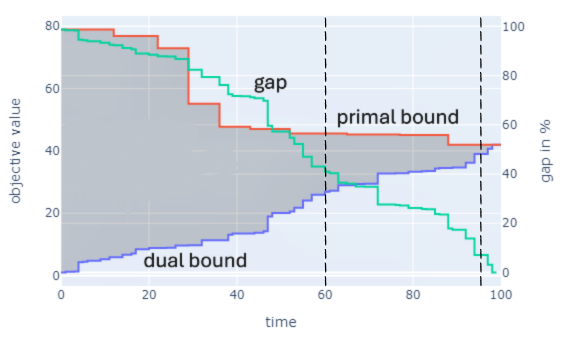
\includegraphics[width=12cm]{ejercicios/gap_gurobi_final.png} 
    \caption{evolución temporal de las cotas y el \textit{gap}. (Fuente: Gurobi)}
\end{figure}

\begin{enumerate}
    \item ¿Qué tipo de problema (\textit{maximizar o minimizar}) se está resolviendo? ¿Por qué?
    \item Indica la expresión que define el \textit{gap}.
    \item ¿Con la información disponible, qué se puede afirmar si se hubiera parado la ejecución en el $t=60$?
    \item ¿Con la información disponible, qué se puede afirmar si se hubiera parado la ejecución en el $t=90$?
\end{enumerate}
